\section{Estratégias de Gestão dos Dados}
\label{sec:gestao}

\subsection{Fontes de dados}
\label{sec:fontes}

O estudo usa apenas dados públicos, resumidos na Tabela~\ref{tab:fontes}. Os dados de operação vêm do ONS, o cadastro de usinas e de geração distribuída vem da Agência Nacional de Energia Elétrica (ANEEL), e os níveis de 2030 vêm de documentos da Empresa de Pesquisa Energética (EPE), do ONS e da Câmara de Comercialização de Energia Elétrica (CCEE). O clima vem da reanálise ERA5 \parencite{hersbach2020,era5_cds}, obtida pela interface da Open-Meteo \parencite{openmeteo}, que não exige cadastro.

\begin{table}[htb]
\centering
\caption{Fontes de dados e uso no estudo.}
\label{tab:fontes}
\footnotesize
\renewcommand{\arraystretch}{1.2}
\setlength{\tabcolsep}{4pt}
\begin{tabularx}{\textwidth}{@{}>{\raggedright\arraybackslash}p{4.1cm}>{\raggedright\arraybackslash}p{3.5cm}>{\raggedright\arraybackslash}X@{}}
\toprule
Fonte & Resolução e período & Uso \\
\midrule
ONS, balanço de energia por subsistema \parencite{ons_dados} & Horária, 2022--2026 & Geração por fonte, intercâmbio e verificação do simulador \\
ONS, carga verificada & 30 min, 2022--2026 & Nível e forma da carga e da geração distribuída \\
ONS, fator de capacidade e geração por usina & Horária, 2022--2026 & Alvos eólico e solar, capacidade e coordenadas das usinas \\
ONS, \textit{constrained-off} & 30 min, eólica desde 2022 e solar desde abril de 2024 & Energia cortada, por motivo \\
ANEEL, SIGA \parencite{aneel_siga} & Cadastro de 01/11/2026 & Pontos de clima e cenários eólicos \\
EPE, PDE 2035 \parencite{epe_pde2035} & Anual & Expansão eólica indicativa e limite de exportação \\
PLAN 2026--2030 \parencite{plan_nt,plan_1rq,plan_2rq} & Anual & Carga, geração distribuída e data centers em 2030 \\
ERA5, via Open-Meteo & Horária, 1995--2026, \NPontosClima{} pontos & Temperatura, vento a 100~m e irradiância \\
IBGE, Censo 2022 \parencite{ibge_censo} & Por estado & Pesos da temperatura das capitais \\
\bottomrule
\end{tabularx}
\end{table}

Entre as fontes, têm DOI a reanálise ERA5, no Copernicus Climate Data Store, e a Open-Meteo, no Zenodo. Os dados do ONS, da ANEEL, da EPE e do IBGE não têm DOI. Nesses casos, a identificação é feita pelo endereço de origem, pela data de coleta e pelo \textit{hash} SHA-256 de cada arquivo, o que permite verificar se uma nova coleta devolve os mesmos dados. Essa verificação é necessária porque os arquivos publicados podem ser revisados pelas instituições.

A coleta foi feita por \textit{scripts}, em \DataColeta, e cada arquivo foi registrado em um manifesto com \NManifesto{} entradas. Uma apresentação da CCEE foi baixada manualmente, pois o servidor recusa o acesso automático, e também consta do manifesto. Os dados brutos, com \VolumeBruto~GB, são mantidos sem alteração. A base de geração distribuída da ANEEL contém dados cadastrais de pessoas físicas, parcialmente ocultados na origem, e por isso só é usada em valores agregados.

\subsection{Reprodutibilidade dos experimentos}
\label{sec:reprodutibilidade}

O processamento é dividido em etapas que leem os arquivos da etapa anterior e gravam os seus em outra pasta, sem modificar as entradas (Figura~\ref{fig:pipeline}). Todas as etapas são executadas em sequência por um único comando, \texttt{python -m src.pipeline}, que parte dos dados brutos e chega às tabelas e figuras em cerca de \TempoPipeline{} minutos. Os \textit{notebooks} não fazem parte dessa sequência.

\begin{figure}[htb]
\centering
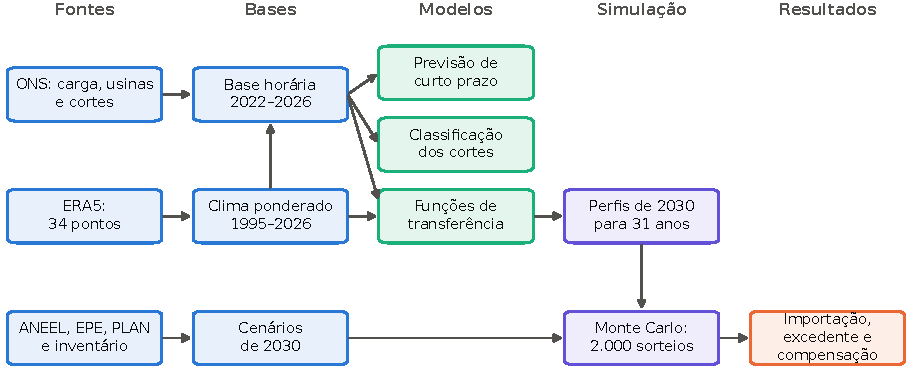
\includegraphics{fig_pipeline}
\caption{Etapas do estudo, das fontes de dados aos resultados.}
\label{fig:pipeline}
\end{figure}

Os cenários e parâmetros ficam em arquivos YAML e CSV separados do código. As versões das bibliotecas estão fixadas, e as sementes aleatórias são \SementeModelos{} para os modelos e \SementeMC{} para a simulação de Monte Carlo. O projeto começou em uma versão de Python e foi transferido para outra (de 3.14 para 3.13), e a simulação de Monte Carlo produziu os mesmos resultados nas duas. Um conjunto de \NTestes{} testes automatizados verifica a conversão de fusos, as unidades, as junções entre bases, o fechamento do balanço e os casos-limite do simulador, como a exigência de que carga adicional nula reproduza o caso sem data centers. As decisões de método estão numeradas e justificadas em um registro com \NDecisoes{} itens.

\subsection{Repositório dos códigos}
\label{sec:repositorio}

% TODO: ao fechar o relatório, incluir o DOI do Zenodo e conferir se o repositório está acessível ao professor.
O código, a configuração, o manifesto e os testes são versionados com Git em \url{https://github.com/MateusMenezes65/estudo-eolica-x-datacenters}. Os arquivos de dados usam Git LFS e podem ser refeitos pelos \textit{scripts} de coleta. Os resultados deste relatório correspondem ao \textit{commit} \texttt{b0ab7fd}.
